\subsection{Seed Synthesizer}

To synthesize seed JavaScript programs, we implement two different
synthesizers: \textit{non-recursive synthesizer} and \textit{built-in function
synthesizer}.
\newline

\subsubsection{Non-Recursive Synthesizer}

The main goal of the non-recursive synthesizer is to cover various cases of
syntax.  It consists of two step: 1) to find the shortest string for each
non-terminal and 2) to synthesize JavaScript programs using the pre-calculated
shortest strings.

\begin{figure}[t]
  \centering
  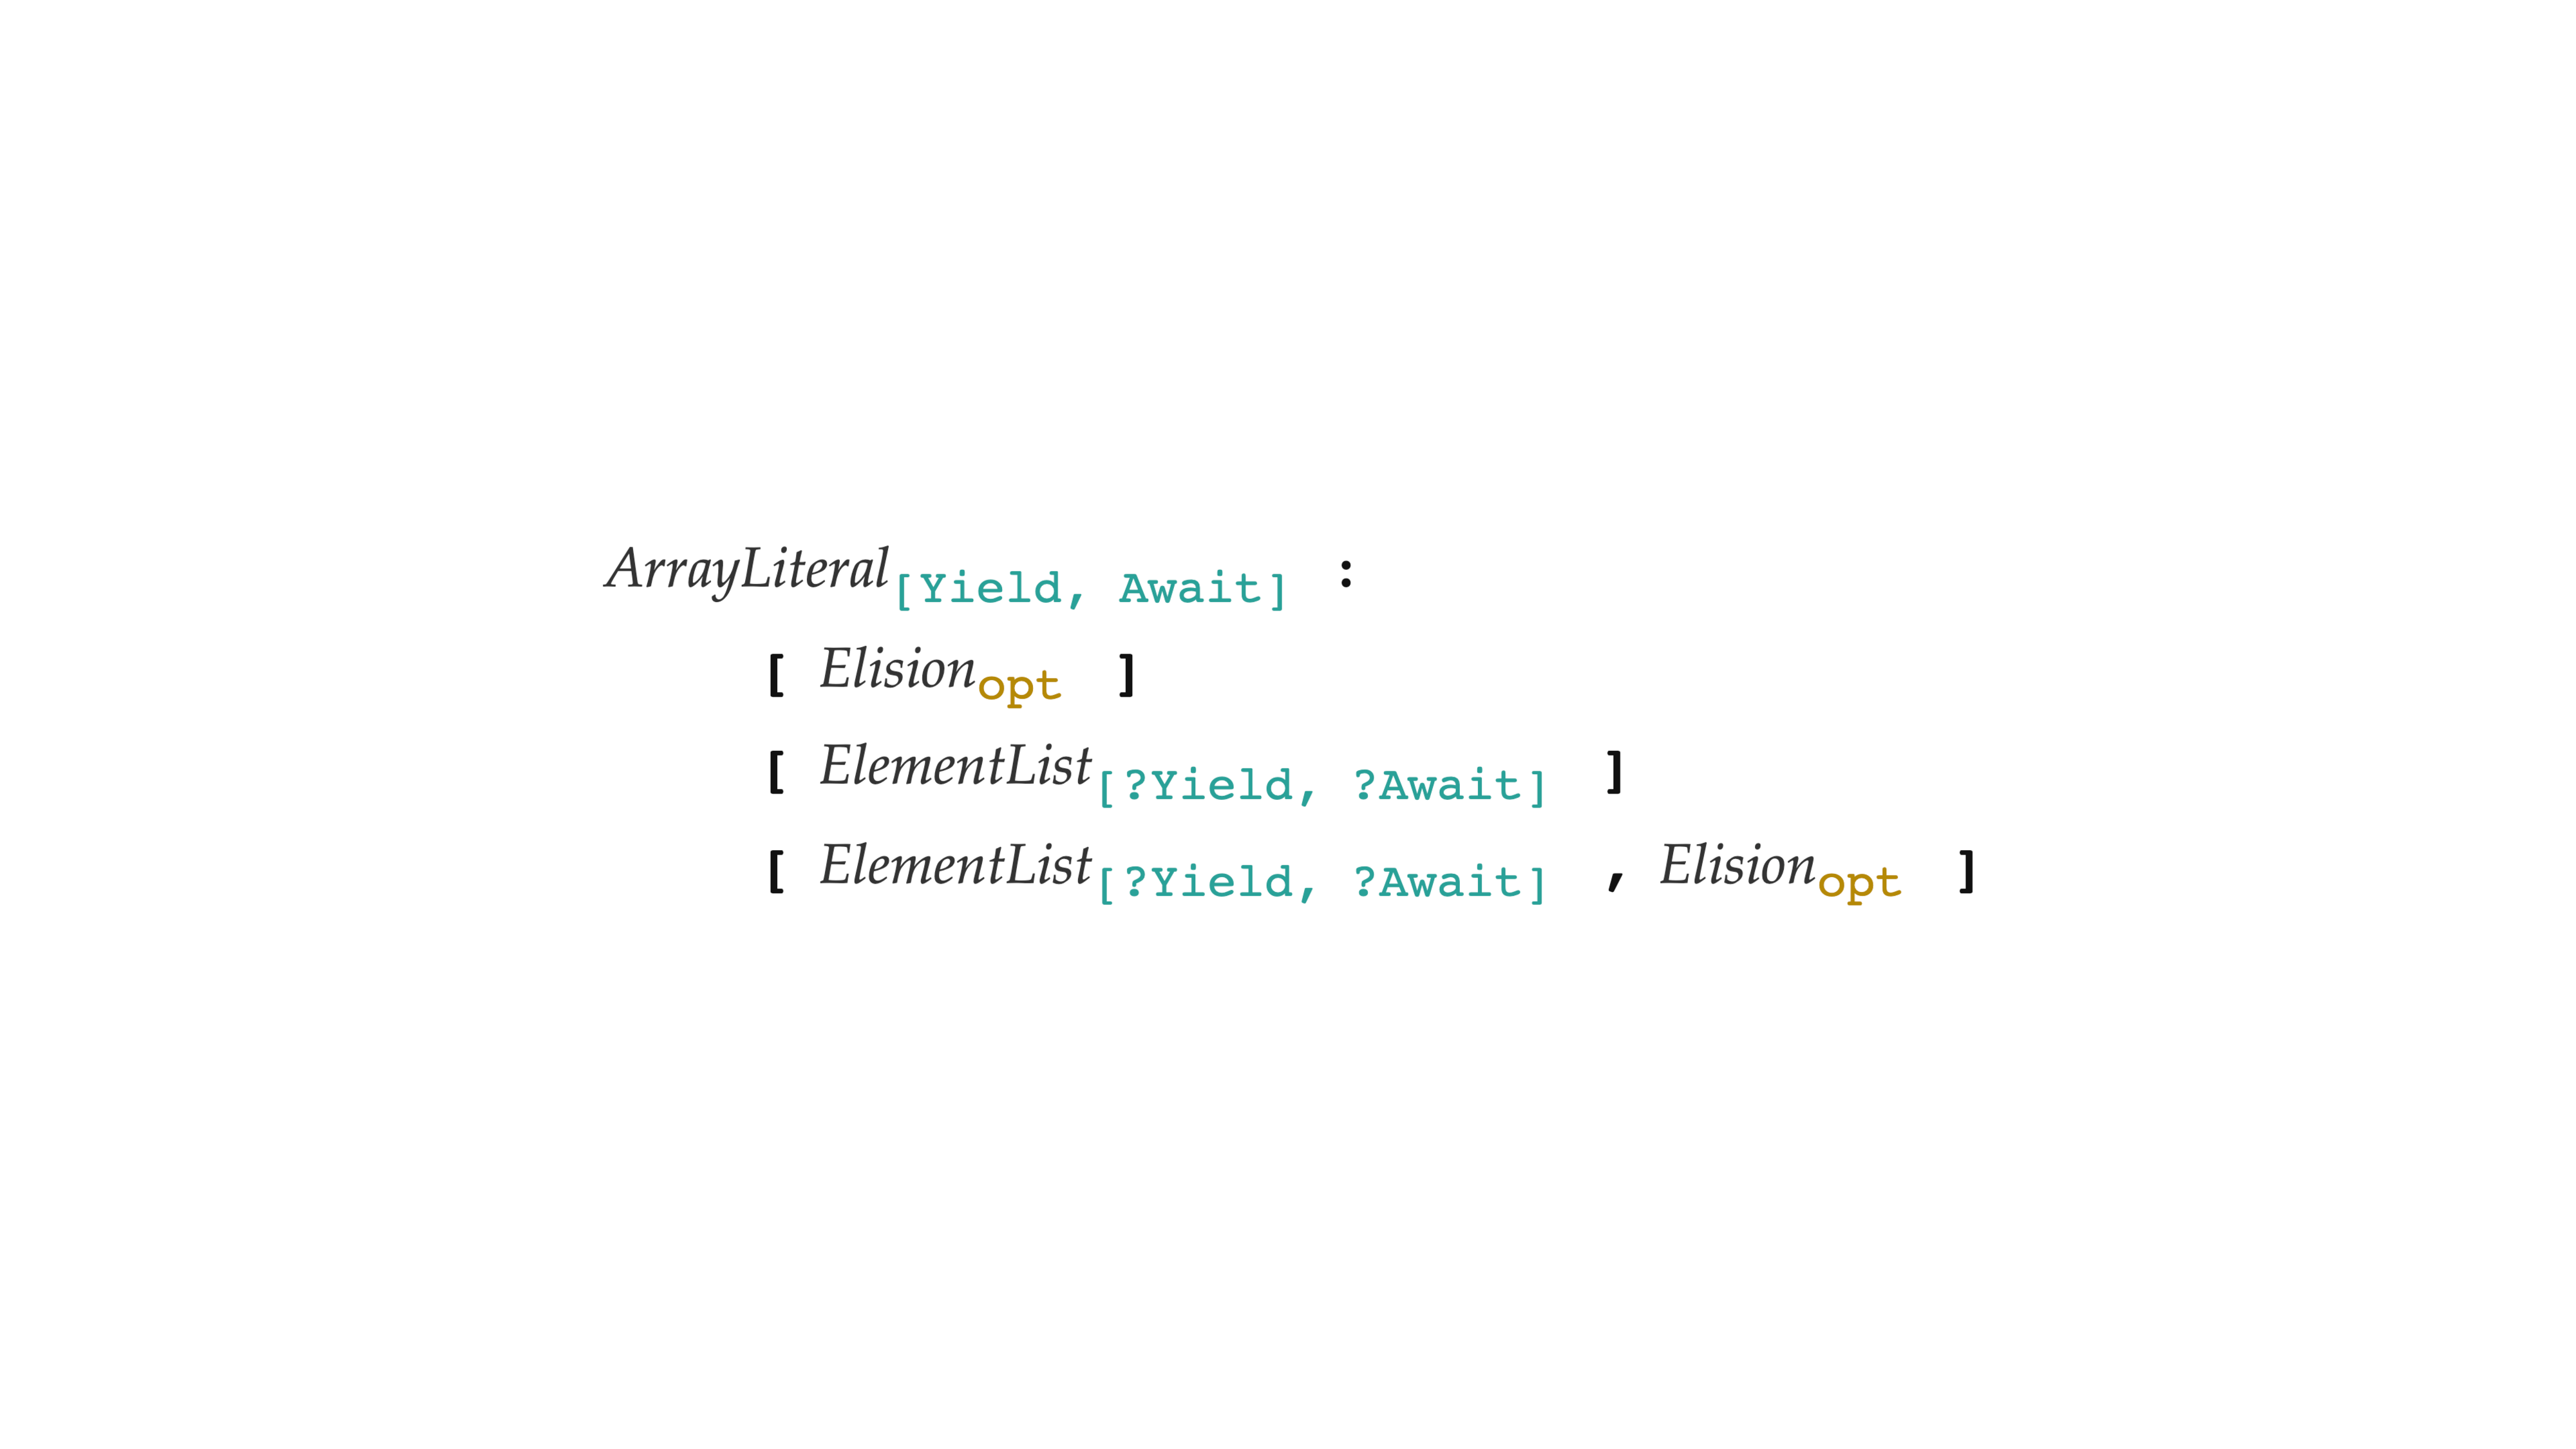
\includegraphics[width=0.42\textwidth]{img/syntax-arrayliteral.pdf}
  \caption{The \textit{ArrayLiteral} production in ES11}
  \label{fig:prod-example}
\end{figure}

\begin{algorithm}[t]
  \caption{Non-Recursive Synthesizer}
  \label{alg:non-rec-synthesizer}
  \begin{algorithmic}
    \STATE \inred{TODO}
    \IF{some condition is true}
      \STATE do some processing
    \ELSIF{some other condition is true}
      \STATE do some different processing
    \ELSE
      \STATE do the default actions
    \ENDIF
  \end{algorithmic}
\end{algorithm}

For the first step, we find the shortest string for each non-terminal.  We
modifies the algorithm introduced by McKenize~\cite{cfg-gen} to find the
shortest string instead of a random string by using a worklist algorithm.
It first finds and stores the shortest strings for base non-terminals not
dependent on other non-terminals and insert non-terminals that utilizes base
non-terminals to a worklist.  A wokrlist is a queue that includes non-terminals
that affected by updated non-terminals.  Then, we remove and get a non-terminal
from the worklist and calculate based on the current information.  If the newly
obtained shortest string is shorter than the original one, we update the
shortest string and push the non-terminals affected by this update to the
worklist.  We repeat this process until the worklist becomes empty.

For example, Figure~\ref{fig:prod-example} shows the \textit{ArrayLiteral}
production in ES11.  Assume that 

\inred{TODO}


\subsubsection{Built-in Function Synthesizer}
\inred{TODO}
